\section{Dynamic Models}

\subsection{Use Case Sequence Diagrams}
\begin{figure}[h!]
	\centering
		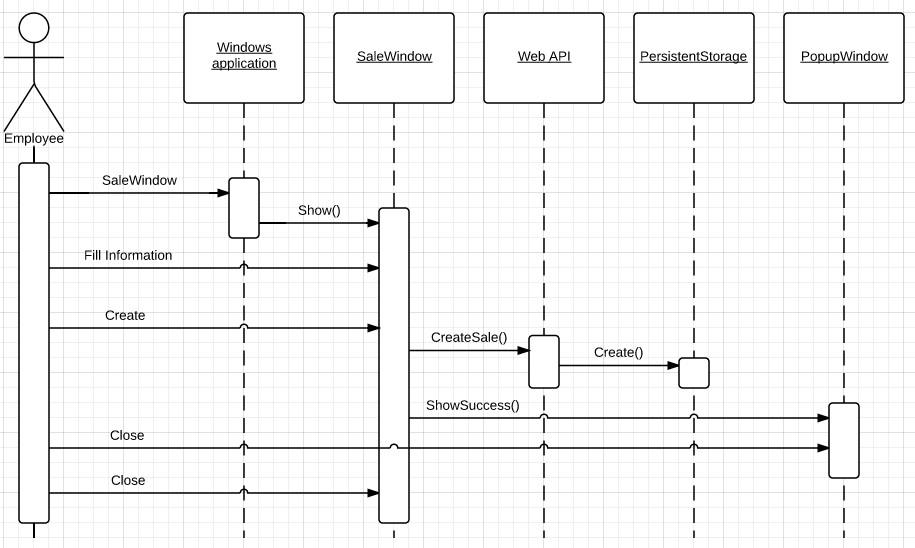
\includegraphics[scale=0.8]{Figures/SequenceDiagram-CreateOrder}\\
		% place the figure in the Figures folder (located with the main file)
		% you need to fix the scale a few times to get it right, but latex does not compress so one can always zoom in to see details.
	\caption{Sequence diagram of the CreateOrder use case.}
  \label{fig:SequenceDiagram-CreateOrder}
  % label it something meanfull
\end{figure}
\begin{figure}[h!]
	\centering
		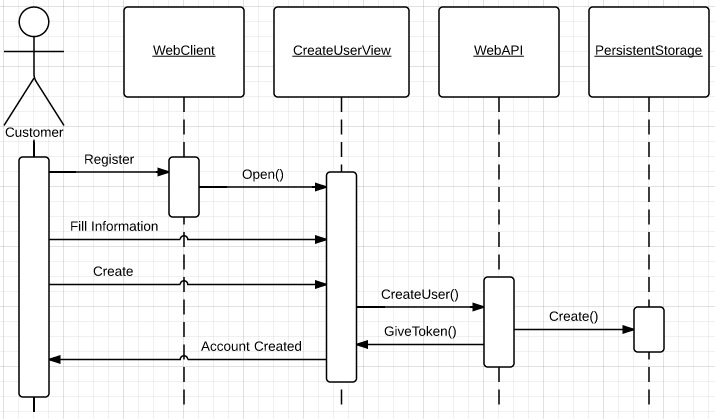
\includegraphics[scale=0.8]{Figures/SequenceDiagram-CreateUserAccount}\\
		% place the figure in the Figures folder (located with the main file)
		% you need to fix the scale a few times to get it right, but latex does not compress so one can always zoom in to see details.
	\caption{Sequence diagram of the CreateUserAccount use case.}
  \label{fig:SequenceDiagram-CreateUserAccount}
  % label it something meanfull
\end{figure}
\begin{figure}[h!]
	\centering
		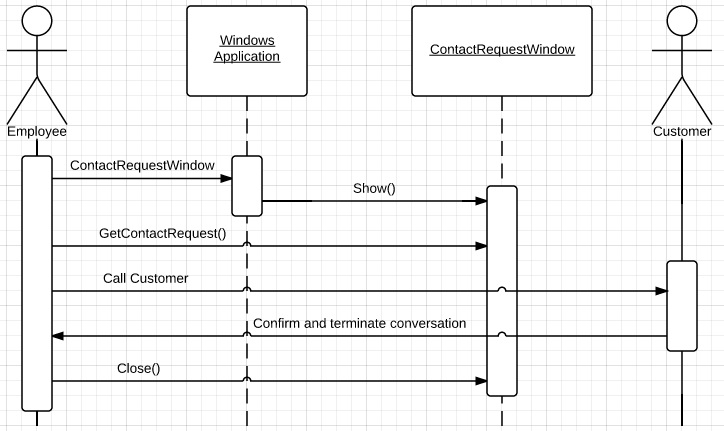
\includegraphics[scale=0.8]{Figures/SequenceDiagram-ContactInterestedCustomer}\\
		% place the figure in the Figures folder (located with the main file)
		% you need to fix the scale a few times to get it right, but latex does not compress so one can always zoom in to see details.
	\caption{Sequence diagram of the ContactInterestedCustomer use case.}
  \label{fig:SequenceDiagram-ContactInterestedCustomer}
  % label it something meanfull
\end{figure}
\begin{figure}[h!]
	\centering
		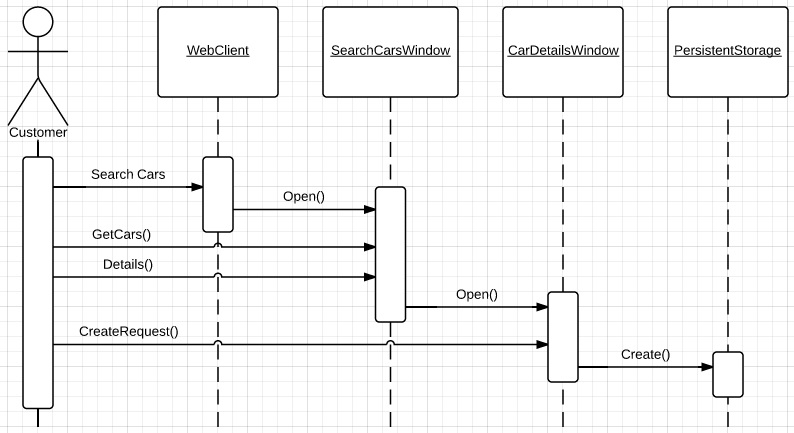
\includegraphics[scale=0.8]{Figures/SequenceDiagram-RequestEmployeeContact}\\
		% place the figure in the Figures folder (located with the main file)
		% you need to fix the scale a few times to get it right, but latex does not compress so one can always zoom in to see details.
	\caption{Sequence diagram of the RequestEmployeeContact use case.}
  \label{fig:SequenceDiagram-RequestEmployeeContact}
  % label it something meanfull
\end{figure}

\subsection{State Diagrams}
\begin{figure}[h!]
	\centering
		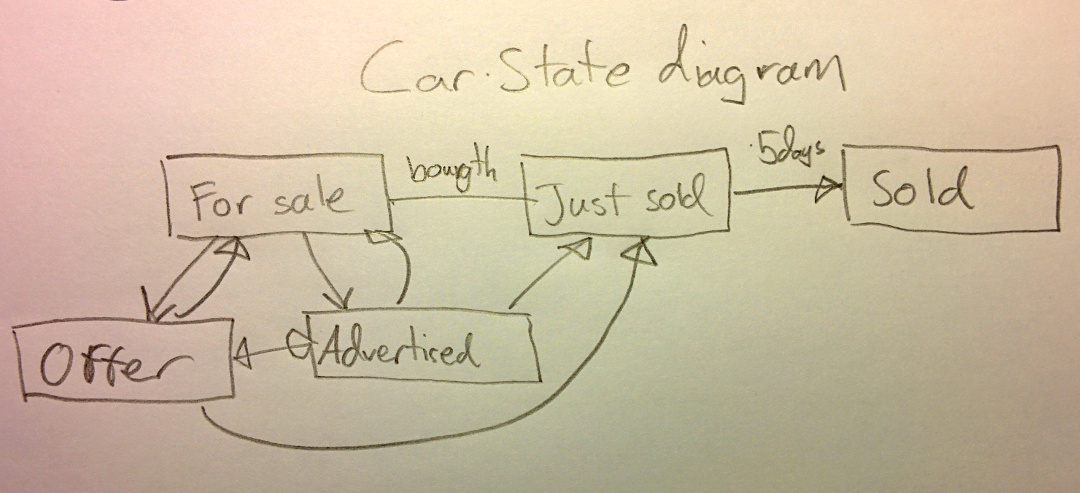
\includegraphics[scale=0.35]{Figures/StateDiagram-Car}\\
		% place the figure in the Figures folder (located with the main file)
		% you need to fix the scale a few times to get it right, but latex does not compress so one can always zoom in to see details.
	\caption{State diagram of the Car object}
  \label{fig:StateDiagram-Car}
  % label it something meanfull
\end{figure}
\begin{figure}[h!]
	\centering
		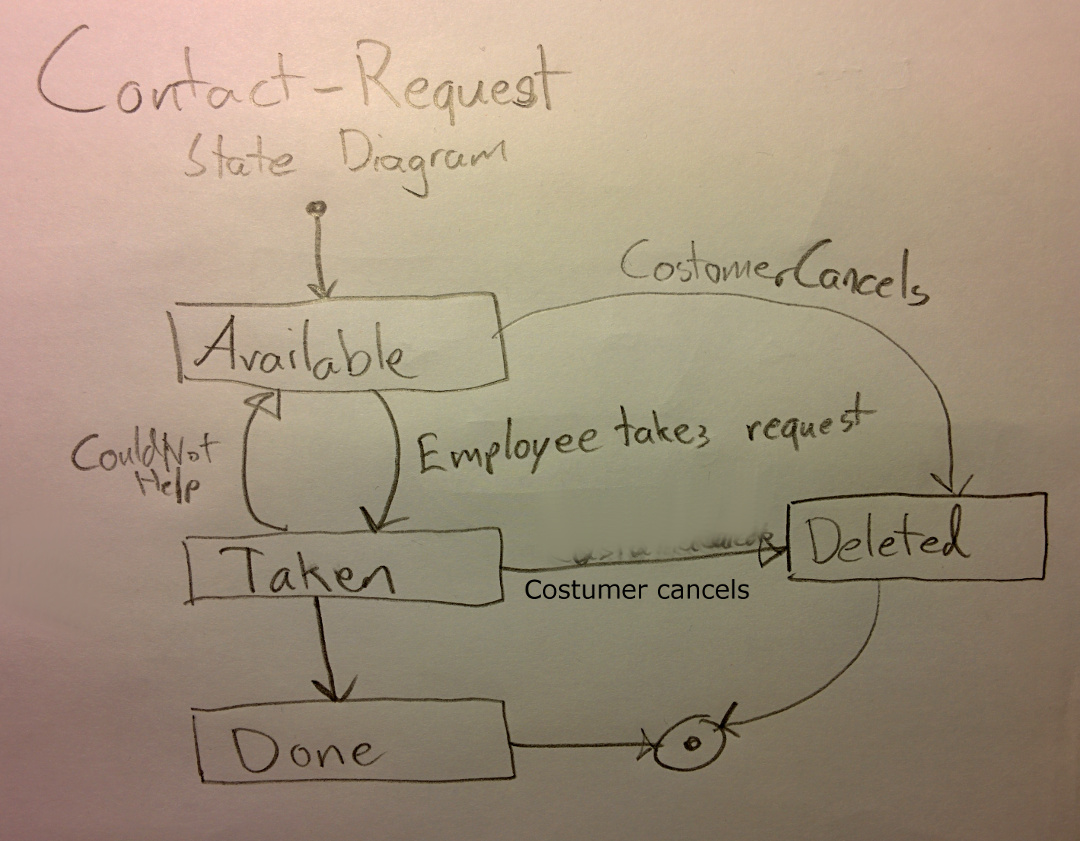
\includegraphics[scale=0.35]{Figures/StateDiagram-ContactRequest}\\
		% place the figure in the Figures folder (located with the main file)
		% you need to fix the scale a few times to get it right, but latex does not compress so one can always zoom in to see details.
	\caption{State diagram of the ContactRequest object}
  \label{fig:StateDiagram-ContactRequest}
  % label it something meanfull
\end{figure}